\documentclass[border=6pt]{standalone}
\usepackage{amsmath}
\usepackage{amssymb}
\usepackage{tikz}
\usepackage{pgfplots}
\pgfplotsset{compat=1.18}
\usetikzlibrary{arrows.meta,calc,positioning}
\begin{document}
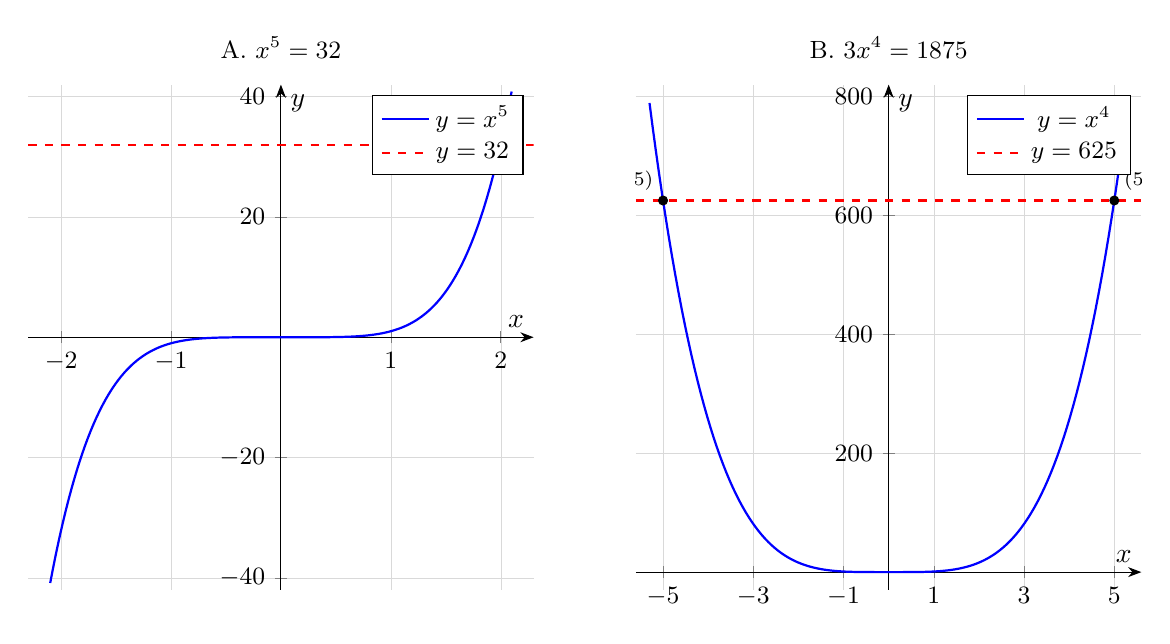
\begin{tikzpicture}
\begin{axis}[name=ax1,
    axis lines = middle,
    xlabel = {$x$}, ylabel = {$y$},
    grid=both,
    grid style={line width=.1pt, draw=gray!30},
    axis line style={-Stealth},
    legend style={font=\small},
    tick label style={font=\small},
    xmin=-2.3, xmax=2.3, ymin=-42, ymax=42,
    xtick={-2,-1,0,1,2},
    ytick={-40,-20,0,20,40},
    width=8cm, height=8cm,
    title={\small A. $x^5=32$},
]
\addplot[domain=-2.1:2.1, samples=150, restrict y to domain=-42:42, thick, blue] {x^5};
\addlegendentry{$y=x^5$}
\addplot[domain=-2.3:2.3, samples=2, thick, red, dashed] {32};
\addlegendentry{$y=32$}
\addplot[only marks, mark=*, mark size=1.6pt, black] coordinates {(2,32)};
\node[anchor=south east, font=\scriptsize] at (axis cs:2,32) {$(2,32)$};
\end{axis}
\begin{axis}[at={(ax1.south east)}, anchor=south west, xshift=1.3cm,
    axis lines = middle,
    xlabel = {$x$}, ylabel = {$y$},
    grid=both,
    grid style={line width=.1pt, draw=gray!30},
    axis line style={-Stealth},
    legend style={font=\small},
    tick label style={font=\small},
    xmin=-5.6, xmax=5.6, ymin=-30, ymax=820,
    xtick={-5,-3,-1,1,3,5},
    ytick={0,200,400,600,800},
    width=8cm, height=8cm,
    title={\small B. $3x^4=1875$},
]
\addplot[domain=-5.3:5.3, samples=150, thick, blue] {x^4};
\addlegendentry{$y=x^4$}
\addplot[domain=-5.6:5.6, samples=2, thick, red, dashed] {625};
\addlegendentry{$y=625$}
\addplot[only marks, mark=*, mark size=1.6pt, black] coordinates {(-5,625) (5,625)};
\node[anchor=south east, font=\scriptsize] at (axis cs:-5,625) {$(-5,625)$};
\node[anchor=south west, font=\scriptsize] at (axis cs:5,625) {$(5,625)$};
\end{axis}
\end{tikzpicture}
\end{document}
